\documentclass[12pt, a4paper]{book}
\usepackage[utf8]{inputenc}
\usepackage[T1]{fontenc}
\usepackage[spanish]{babel}

\setlength{\parindent}{2mm}		%identacion del parrafo
\setlength{\parskip}{5mm}		%separacion entre parrafos
\usepackage[lmargin=2.0cm,rmargin=2.0cm,top=3.5cm,bottom=3.5cm]{geometry}
\usepackage{hyperref}
\usepackage{graphicx}
\usepackage{float} 
%\usepackage{subcaption}
\usepackage{multicol}
\usepackage{amsfonts}
\usepackage{physics}
\graphicspath{{imagenes/}}
\usepackage{amsmath}


\setlength{\tabcolsep}{20pt}
\renewcommand{\arraystretch}{1.5}


\title{Machine Learning.}
\date{\today}
\author{Angel Chaico\\Facultad de ciencias, 
	UNI\thanks{yo}
	\and yo}

\begin{document}
	\maketitle
	\tableofcontents
	
\chapter{aora}
random forest, neural network, regresion logisticy hacer bibliografi por capitulo.\\

En loc codigos iran ejemplos graficos de cada modelo aplicado.

\part{Statistical and probabiliti (EDA).}
\begin{figure}[H]
	\centering
	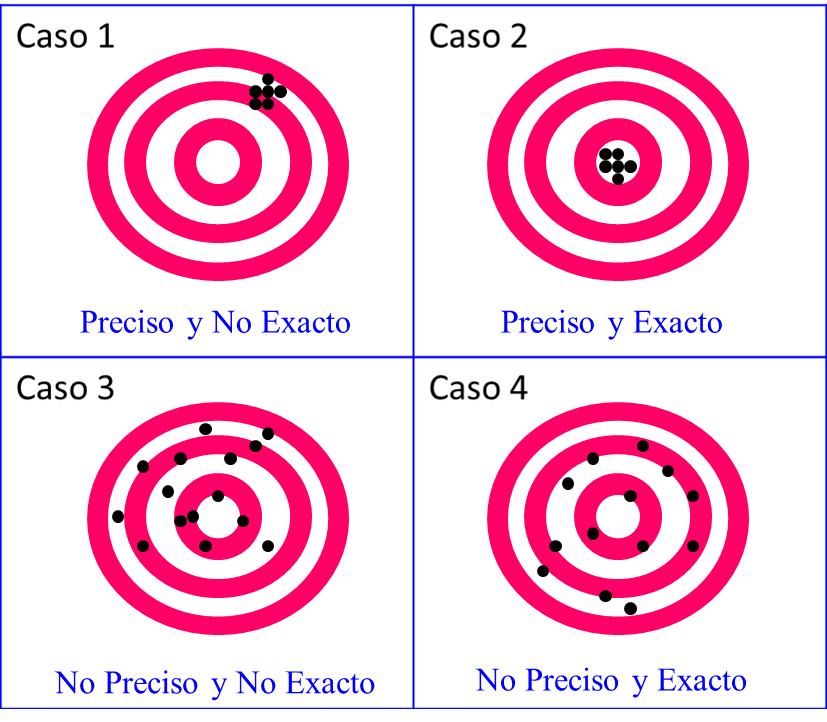
\includegraphics[scale=0.5]{exacto.png}
\end{figure}
\begin{figure}[H]
	\centering
	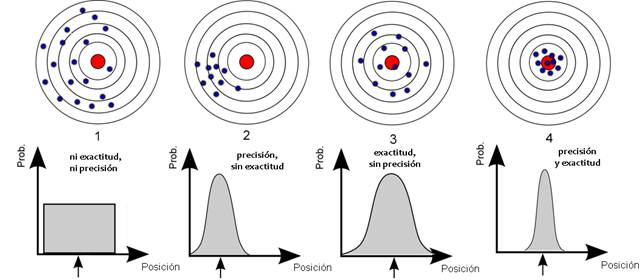
\includegraphics[scale=0.5]{presicion.jpg}
\end{figure}
\section{Estimates and explorind data.}
\section{Distributions.}
\section{Statistical experiment.}



\part{Resamplin(train and test set).}

\chapter{Sampli:stratied}

\chapter{Imbalance data.}

\section{Undersampling}

\section{Oversamplig}
\subsection{Bootstraping}
\subsection{data generation: SMOTE algorithm}
\section{Weighting.}
\section{Cost-based classification.}


\section{bibliografi} 
\href{https://www.analyticsvidhya.com/blog/2016/03/practical-guide-deal-imbalanced-classification-problems/}{revisar}\\
practical sttistical for data science, by peter bruce.\\


\part{Supervised (model)}
\chapter{Linear regression.}

\chapter{Logistic regression.}
\section{Regularization.}
\section{Código.}

\chapter{Desicion tree.}


\section{regression}:
\begin{itemize}
	\item We divide the predictor space- that is, the set of posible values for $X_1, X_2, \cdots ,X_p$- into $J$ distinct and non-overlapping regions, $R_1,R_2,\cdots ,R_J$.
	\item For every observation that falls into the region $R_j$, we make the same prediction, which is simply the mean of the response values for the training observations in $R_j$.
\end{itemize}
The goal es to find $R_1,\cdots,R_J$ that minimize the RSS given by:
\begin{equation}
	\sum_{j=1}^{J}\sum_{i \in R_j}(y_i-\hat{y}_{R_j})^2
\end{equation}
Recursive binary splitting, we seek the value of j and s that minimize the equation
\begin{equation}
	\sum_{i:x_i\in R_1(j,s)}(y_i-\hat{y}_{R_1})^2+\sum_{i:x_i\in R_2(j,s)}(y_i-\hat{y}_{R_2})^2
\end{equation}
Cost complexity pruning (weakest link pruning). For each value of  $\alpha$ there corresponds a subtree $T\in T_0$, $T_0$ is when $\alpha=0$, such that is as small as possible. The $\abs{T}$ indicate the number of terminal nodes of the tree $T$.
\begin{equation}
	\sum_{m=1}^{\abs{T}}\sum_{i:x_i\in R_m} (y_i-\hat{y}_{R_m})^2 +\alpha \abs{T}
\end{equation}

\begin{figure}[H]
	\centering
	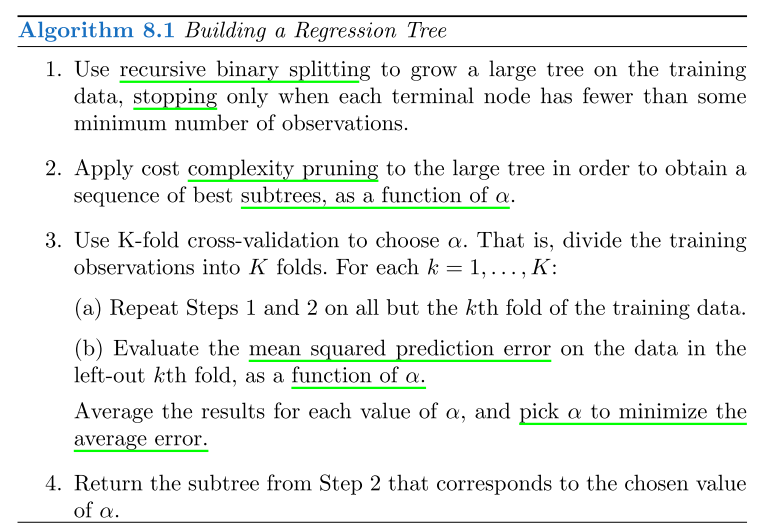
\includegraphics[scale=0.5]{regressionTree.png}
	\caption{Although CV error is computed as a function of $\alpha$, it is convenient to display the result as a function of $\abs{T}$.}
\end{figure}
\section{Classification} 
\textbf{Tree vs linear}

\chapter{Random Forest.}
When building desicion trees, each time a split in a tree is considered, a random sample of m predictor is chosen as split candidates from the fulll set of p predictors (decorrelating trees).
\section{Regularization.}
\begin{itemize}
	\item As with bagging, random forests will not overfit if we increase B trees, so in in practis we use a value of B sufficiently large for the error rate to have settled down.
\end{itemize}
\begin{table}[H]
	\centering
	\begin{tabular}{|c|c|c|}
		\hline 
		Metod & default & observation \\
		\hline 
		random sample of m predictors & m = $\sqrt{p}$ & \\
		\hline 
		bootstrapped (max\_sample) &&\\
		\hline
		Out-of-bag (OOB)&&\\
		\hline
		criterion &gini&\\
		\hline 
		max depth &&\\
		\hline 
	\end{tabular}
\end{table}
\section{Código.}
Importance attributes
\begin{table}[H]
	\centering
	\begin{tabular}{|c|c|}
		\hline
		feature\_importances\_&\\
		\hline 
		n\_outputs\_&\\
		\hline 
	\end{tabular}
\end{table}

Observactiona
\begin{itemize}
	\item  Para cada X\_train diferente se obetiene features importances diferentes en el modelo resultalte, como determinar las features importances si el modelo cambia al cambiar los X\_train?
\end{itemize}
\chapter{Bagging}
\chapter{Boosting.}
\chapter{Bayesian additive regression trees.}



\chapter{Supert Vector Machine.}
\section{Regularization.}
\section{Código.}

\part{Unsupervised (model)}
\chapter{K-means}
\chapter{Hierarchical Clustering.}


\part{Deep learning (model)}

\chapter{Neural Networks}

\section{Activation function.}
\subsection*{Sigmoid}
\subsection*{ReLU}
\subsection*{ELU}

\begin{equation}
	ELU_{\alpha}=\begin{cases}
		\alpha (e^z-1)&, z<0\\
		z&, z\geq 0
	\end{cases} 
\end{equation}

\section{Convulation layer.}
\section{Poling layer.}


\chapter{Regularization.}
Problems:
\begin{itemize}
	\setlength\itemsep{0.1em}
	\item Vanishing gradient or exploding gradients.
	\item Not have enought trainig data.
	\item Slow.
	\item Overfitting.
\end{itemize}

\section{The Vanishing/Exploring gradients}

\subsection*{Glorot and He initialization}
Glorot and Yoshua show the with logistic sigmoid function activation and weight initialization technique, the variance of the output of each layer is much greater than the variance of its inputs.

Glorot show that the connection weights of each layer must be initialized randomly as\footnote{fan\_in is the number of input and fan\_out the number of neuron of the layer}:
\begin{eqnarray}
	\text{Normal distribution} , \mu =0, \sigma^2 =\frac{1}{fan_{avg}}\\
	\text{Uniform distribution between}-r,r\text{ with } r=\sqrt{\frac{1}{fan_{avg}}}\\
	fan_{avg}=\frac{fan_{int}+fan_{out}}{2}
\end{eqnarray}

\begin{table}[H]
	\centering
	\begin{tabular}{c|c|c}
		\hline 
		initialization & activation function & $\sigma^2(Normal)$\\
		\hline 
		Glorot & None, tanh, logistic, softmax&$\frac{1}{fan_{avg}}$\\
		He&ReLU and variant&$\frac{2}{fan_{int}}$\\
		Lecun&SELU&$\frac{1}{fan_{int}}$\\
		\hline 
	\end{tabular}
	\caption{Initialization parameters for each type of activation function; $r=\sqrt{3\sigma^2}$.}
\end{table}


\begin{verbatim}
	keras.layers.Dense(10,, activation="relu", kernel_initializer="he_normal")
\end{verbatim}

\begin{verbatim}
	% fan_in->fan_avg
	he_avg_init=keras.initializers.VarianceScaling(scale=2,mode="fan_avg")
	keras.layers.Dense(10, activation="sigmoid", kernel_initializer=he_avg_init)
\end{verbatim}

\subsection*{Nonsaturing Activation Function}
Glorot and Bengio show that the problems with unstable gradients were in part due to a poor choice of activation function.
\begin{itemize}
	\item \textbf{ReLU}, problem dying ReLU.
	\item \textbf{leaky ReLU}, $LeakyReLU_{\alpha}(z)=max(\alpha z,z)$, usual fixed $\alpha =0.01$, from one paper, it conclusions was that the leaky variants always outperform the estric ReLU, $\alpha =0.2$ seemed to resutl in better performance. 
	\item \textbf{RReLU},randomize leaky ReLU, $\alpha$ is random during the training and fixed to an average value during testing; seems to act regularizer reducing the overfitting of the training set.
	\item \textbf{PReLU}, parametric leaky ReLU, $\alpha$ to be learned during training; was reported to strongly outperform ReLU on large image datasets, but on smaller it runs the risk of overfitting the training set.
	\item \textbf{ELU} exponential linear unit, better that all varians ReLU. ELU network will be sslower than a ReLU network.
	\item \textbf{SELU}, Scaled ELU, in stack of dense layer result self-normalize: the output of each layer will tend to preserve a mean of 0 and standar desviation of 1 during trainig, which solve the grading problem. condiction:input staandarized 0,1; initialized with LeCu; architecture must be sequential,all layer must be dense
\end{itemize}
\begin{verbatim}
	keras.layers.Dense(10, kernel_initializer="he_normal")
	keras.layers.LeakyReLU(alpha=0.2)\PReLU()
	%
	keras.layers.Dense(10, activation="selu", kernel_initilizer="lecun_normal")
	
\end{verbatim}

\subsection*{Bach Normalization}
The before not guarantee that gradient come back during trainig. Sergey and Christian proposed BN, consist of adding an operation in the model just before of after the activation fuction of each hidden layer. The algorithm needs to estimate each input's mean and standar desviation (does over mini-bach)
\begin{eqnarray}
	\mu_B=\frac{1}{m_B}\sum^{m_B}_{i=1}x^{(i)}\\
	\sigma^{2}_B=\frac{1}{m_B}\sum_{i=1}^{m_B}\left(x^{(i)-\mu_B}\right)^2\\
	\hat{x}^{(i)}=\frac{x^(i)-\mu_B}{\sqrt{\sigma^{2}_B}+\epsilon}\\
	z^{(i)}=\gamma \cdot \hat{x}^{(i)}+\beta 
\end{eqnarray}
$\gamma$ (outputscaler vector), $\beta$ (output offset vector) are learned through regular backpropagation, and $\mu$ (the final input mean vector) and $\sigma$ (the final  input standar desviation vector) are stimated using an exponential moving average (estimed during training but used after).

The vanishing gradients problem was strongly reduced; BN acts like a regularizer; there is a runtime penalty (evoiding updating the previos layer's weight and biases).

The aoutor of the BN paper arqued in favor of adding the BN layers before the activation function, rather than after. There is some debate about this, as which is preferable seems to depend on the task. Since BN layer include one offset parameter per input, you can remove the bias term from the previos layer.

\textbf{momentum} this parameter is used by the BN layer when it updates the exponential moving averages.

BN has become one of the most-used layers in deep neural networks.\footnote{Now fixed-updated by Hogyi Zhang is view recently}
\begin{verbatim}
	model = keras.models.Sequatial([
	keras.layers.Flatten(input_shape=[28,28]),
	keras.layers.BatchNormalization(),
	keras.layers.Dende(300, kernel_initializatizer="he_normal", use_bias=False),
	keras.layers.BatchNormalization(),
	keras.layers.Activation("elu")
	keras.layers.Dende(100, kernel_initializatizer="he_normal", use_bias=False),
	keras.layers.BatchNormalization(),
	keras.layers.Activation("elu"),
	keras.layers.Dense(10, activation="sofmax")
	])
\end{verbatim}
\subsection*{Gradient Clipping}
\begin{verbatim}
	optimizer= keras.optimizers.SGD(clipvalue=1.0)
	model.compile(loss="mse", optimizer=optimizer)
\end{verbatim}

\section{Reusing Petrained Layer}

\section{Faster Optimizationers.}

\section{Overfitting.}
Even though Batch Normalization was designed to solve the unstable gradients problems, it also acts like a pretty good regularizer.
\subsection*{L1,L2 regularization}
\begin{verbatim}
	layer = keras.layers.Dense(100, activation="elu", kernel_initializer="he_normal",
	kernel_regularizer=keras.regularizers.l2(0.01))	
\end{verbatim}

\begin{verbatim}
	from functools import partial
	RegularizedDense = partial(
	keras.layers.Dense,
	activation="elu",
	kernel_initializar="he_normal",
	kernel_regularizer=keras.regularizers.l2(0.01)
	)
	model = keras.models.Sequential([
	keras.layers.Flatten(input_shape=[28,28]),
	RegularizedDense(300),
	RegularizedDense(100),
	RegularizedDense(10,activation="softmax",
	kernel_initializer="glorot_uniform")
	])
\end{verbatim}

\subsection*{Dropout}
At every training step, every neuron(including the input neurons, but always excluding the output neurons) has a probability $p$ of being temporarily "dropped out", meaning it will be entirely ignored during this training step, but it may be active during the next step. The hyperparameter p is called the dropout rate, and it is typically set between $\%10-\%50$. The state-of-the-art neural networks get $1-2\%$ accuracy boost simply by adding dropout. Also. we need to multiply each input connection weight by the keep probability (1-p) after training. Alternatively, we can divide each neuron's output by the keep probability during training(don't equvalent but they work equally well).
\begin{verbatim}
	model = keras.model.Sequential([
	keras.layers.Flatten(input_shape=[28,28]),
	keras.layers.Dropout(rate=0.2),
	keras.layers.Dense(300, activation="elu",kernel_initializer="he_normal"),
	keras.layers.Dropout(rate=0.2),
	keras.layers.Dense(100, activation="elu", kernel_initializer="he_normal"),
	keras.layers.Dropout(rate=0.2),
	keras.layers.Dense(10,activation="softmax")
	
	])
\end{verbatim}
If you observed that the model is overfitting, you can increase the dropout rate.Conversly, you should try decreasing the dropout rate if the model  underfits the training set. It can also help to increase the dropout rate for large layers, and reduce it for small ones. Moreover, many state-of-the-art architectures only use dropout after the last hidden layer, so you may want to try this if full dropout is too strong. Dropout does tend to significanty slow down convergence, but it usually result in a much better model when tuned properly. So, it is in generally well worth the extra time and effort.

\textbf{observation} Dropout is only active during training, made sure to evaluate the training loss without the dropout (after training).

\subsection*{MC Dropout}
\subsection*{Max-Norm Regularization.}


\section{Summary} 
\begin{table}[H]
	\centering
	\begin{tabular}{|c|c|}
		\hline
		Lasso, Ridge, slow learning $\lambda$ & tunning parameter\\
		\hline
		dropout learning & remove fraction of unit per layer and scaler weight\\
		\hline
		early stopping, epoch, batch size& details of stochastic gradient descent\\
		\hline 
		number of layer, and unit fro layer& \\
		\hline 
	\end{tabular}
\end{table}

\section{bibliografy}
2014 paper Nitish Srivastava (dropout)\\



\part{Optimization (opt model).}
\chapter{First order methods.}
\section{Adagrad.}
\section{Adam.}

\chapter{Second order methods.}
\section{Newton's method.}
\section{Secant method.}

\chapter{Direct Methods.}
\section{Nelder-mead simplex method.}

\chapter{Stochastic methods.}
\section{Noise descent.}
\section{Cross-Entropy  method.}



\part{Regularization (overfitting).}

\part{Metrics (evaluation)}
\chapter{Regression}

\chapter{Classification}
\begin{itemize}
	\item Confusion matrix
	\item ROC.
	\item PR
	\item Gain and lift chart.
\end{itemize}
\section{Matrix confusion}
Fundamentally, the assessment  process atempts to learn which model produces the most accurate and \underline{useful predictions}.

When 1s are rare, the ratio of false positives to all predicted positives can be high, leading to the unintuitive situation in which a predicted 1 is most likely a 0.\footnote{Default desicion point or cutoff is 0.5}

In \underline{inbalance classes} the rare class is usually the class of more interestet and is typically designed 1, in contrast to \underline{more prevalent 0s}. The 1s are the more important case, in the sense that misclassifying them as 0s is costlier than misclassifying 0s as 1s (exp legitimate insurance claims 0, fraudulent 1). The most accurate classification model may be one that simply classifies everything as a 0.
\begin{figure}[H]
	\centering 
	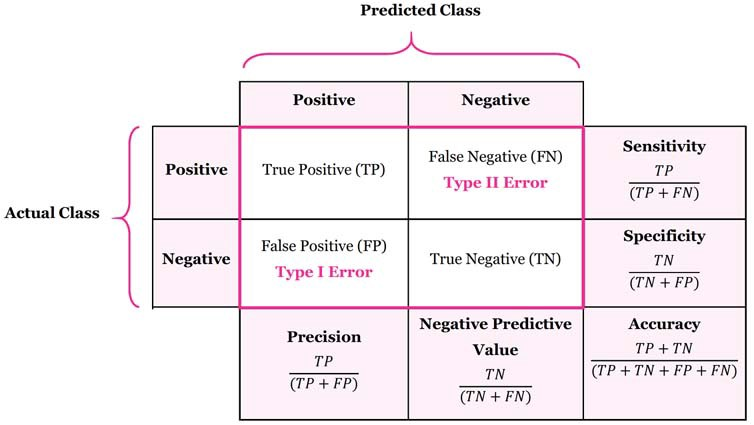
\includegraphics[scale=0.5]{recall.jpg}
	\caption{Matrix cunfusion, sensitivity is recall.}
\end{figure}


\section{ROC curve.}
The Geometric Mean or G-Mean is a metric for imbalanced classification that, if optimized, will seek a balance between the sensitivity and the specificity.
\begin{equation}
	G-mean=\sqrt{Sensitivity \cdot Specificity}
\end{equation}
Given that we have already calculated the Sensitivity (TPR) and the complement to the Specificity when we calculated the ROC Curve, we can calculate the G-Mean for each threshold directly.

It turns out there is a much faster way to get the same result, called the Youden’s J statistic.
\begin{equation}
	J = Sensitivity + Specificity – 1
\end{equation}
We can then choose the threshold with the largest J statistic value
\begin{figure}
	\centering
	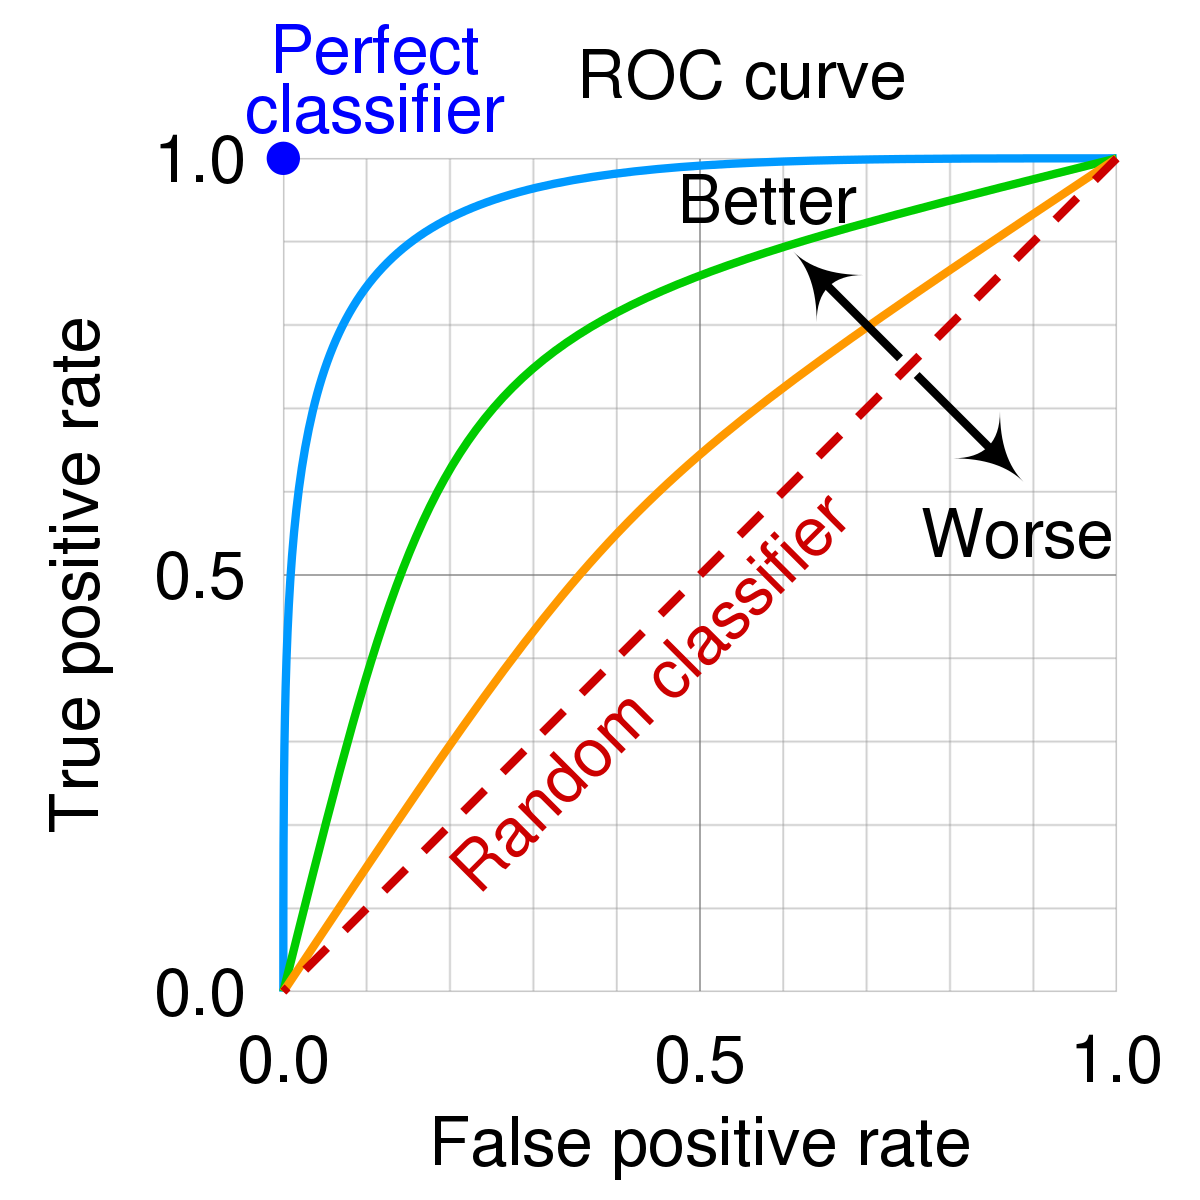
\includegraphics[scale=0.2]{ROC.png}
	\caption{If ROC (sensity-recall) hugs the upperleft corner it will identify lots of 1s without misclassifying  lots of 0s as 1s. Prevalence is y=1 / total. false positive rate is 1-specifity.}
\end{figure}
\begin{figure}[H]
	\centering
	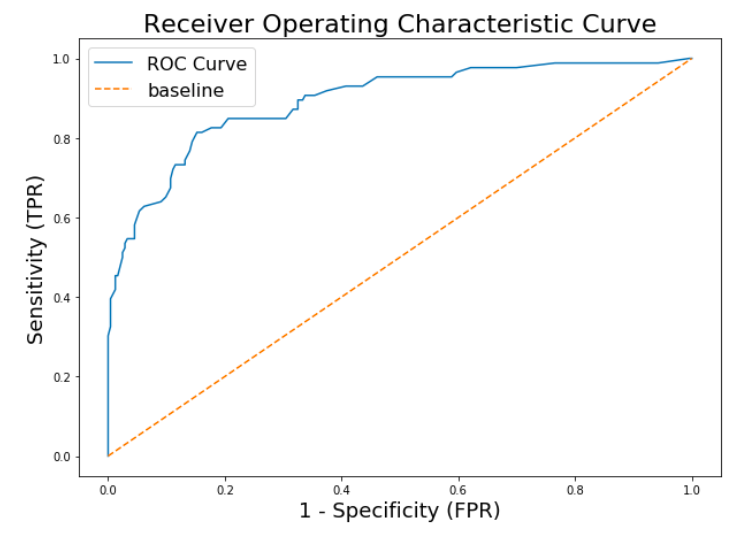
\includegraphics[scale=0.5]{ROC2.png}
\end{figure}

\section{PR curve}
PR curves are specially useful in evaluating data with highly unbalanced out-comes.
\begin{figure}[H]
	\centering
	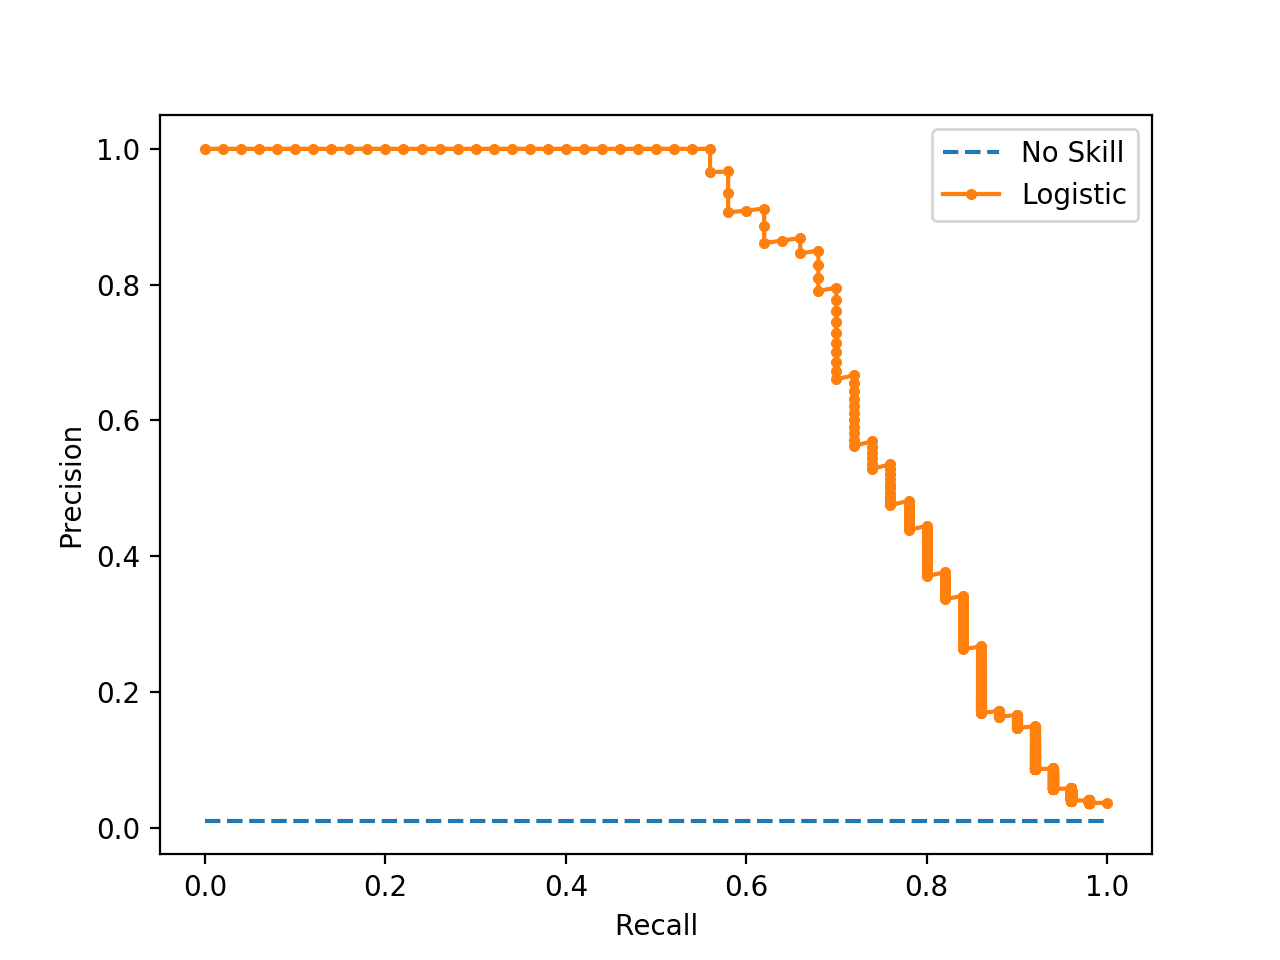
\includegraphics[scale=0.2]{PR}
	\caption{}
\end{figure}
Fuentes \href{https://machinelearningmastery.com/threshold-moving-for-imbalanced-classification/}{A Gentle Introduction to Threshold-Moving for Imbalanced Classification}

If we are interested in a threshold that results in the best balance of precision and recall, then this is the same as optimizing the F-measure that summarizes the harmonic mean of both measures.
\begin{equation}
	F-Measure = \frac{(2 \cdot Precision \cdot  Recall) }{(Precision + Recall)} 
\end{equation}
first calculates the F-measure for each threshold, then locates the score and threshold with the largest value.

\section{Gain chart and lift chart.}
Gain and Lift charts are two approaches used while solving classifications problems with imbalanced data sets. The gain chart and lift chart is the measures in logistic regression that will help organizations to understand the benefits of using that model.\href{http://mlwiki.org/index.php/Cumulative_Gain_Chart}{Cumulative Gain Chart}
\begin{equation}
	Gain=\frac{CumulativeNumberOfPositiveObservationsUptodecibels}{TotalNumberOfPositiveObservationInData}
\end{equation}
\begin{figure}[H]
	\centering
	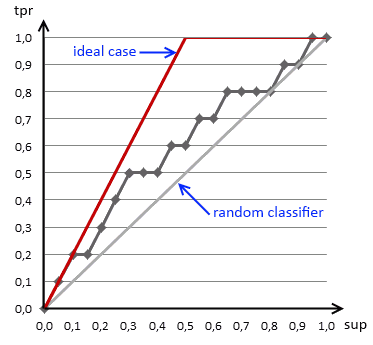
\includegraphics[scale=0.5]{gain_chart.png}
\end{figure}
it says how much population we should sample to get the desired sensitivity of our classifier
i.e. if we want to direct 40\% of potential repliers to our targeting campaign, we should select 20%
\begin{figure}[H]
	\centering
	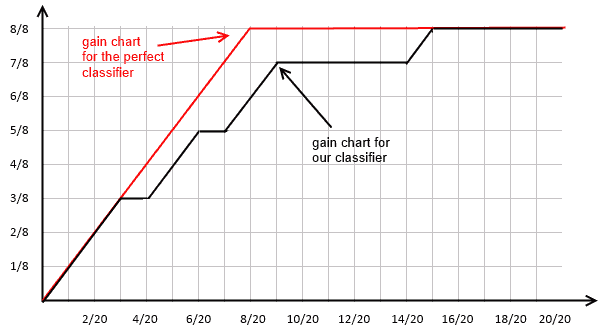
\includegraphics[scale=0.5]{gain2.png}
\end{figure}
\begin{figure}[H]
	\centering
	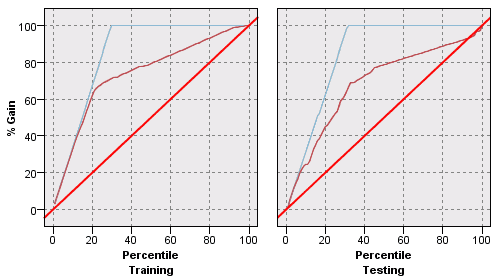
\includegraphics[scale=0.5]{gain3.png}
	\caption{we can easily see if a classifier overfits on the test set, but underperforms on the testing}
\end{figure}

\begin{equation}
	lift = \frac{Cumulative number of positive observations upto decile i using ML model}{Cumulative Number of Positive Observations upto Decile i using Random Model.}
\end{equation}
falta analisar el lift, el libro donde encontre es el data mining for eider franck, revisar luego, usare lo mencionado en ROC, PR y el tratamiendo de datos no balanceados por mietras, el lift es para saber los costos, vere mas adelante.

\section{K-S Chart}

\section{bibliografia.}
\href{https://machinelearningmastery.com/threshold-moving-for-imbalanced-classification/}{A Gentle Introduction to Threshold-Moving for Imbalanced Classification}\\
\href{http://mlwiki.org/index.php/Cumulative_Gain_Chart}{Cumulative Gain Chart
}\\
Practical statistical for data sicience, peter bruce and andrew bruce\\



\part{Python.}
\chapter{sklearn.preprocessing}
Preprocessing and Normalization\\
The sklearn.preprocessing module includes scaling, centering, normalization, binarization methods.
\begin{itemize}
	\item sklearn.preprocessing.StandardScaler().
	\begin{equation}
		\frac{x_i-mean(x)}{sd(x)}
	\end{equation}
	\item sklearn.preprocessing.MinMaxScaler().
	\begin{equation}
		\frac{x_i-min(x)}{max(x)-min(x)}
	\end{equation}
	\item sklearn.preprocessing.RobustScaler().
	\begin{equation}
		\frac{x_i-Q_1(x)}{Q_3(x)-Q_1(x)}
	\end{equation}
\end{itemize}

\begin{figure}[H]
	\centering
	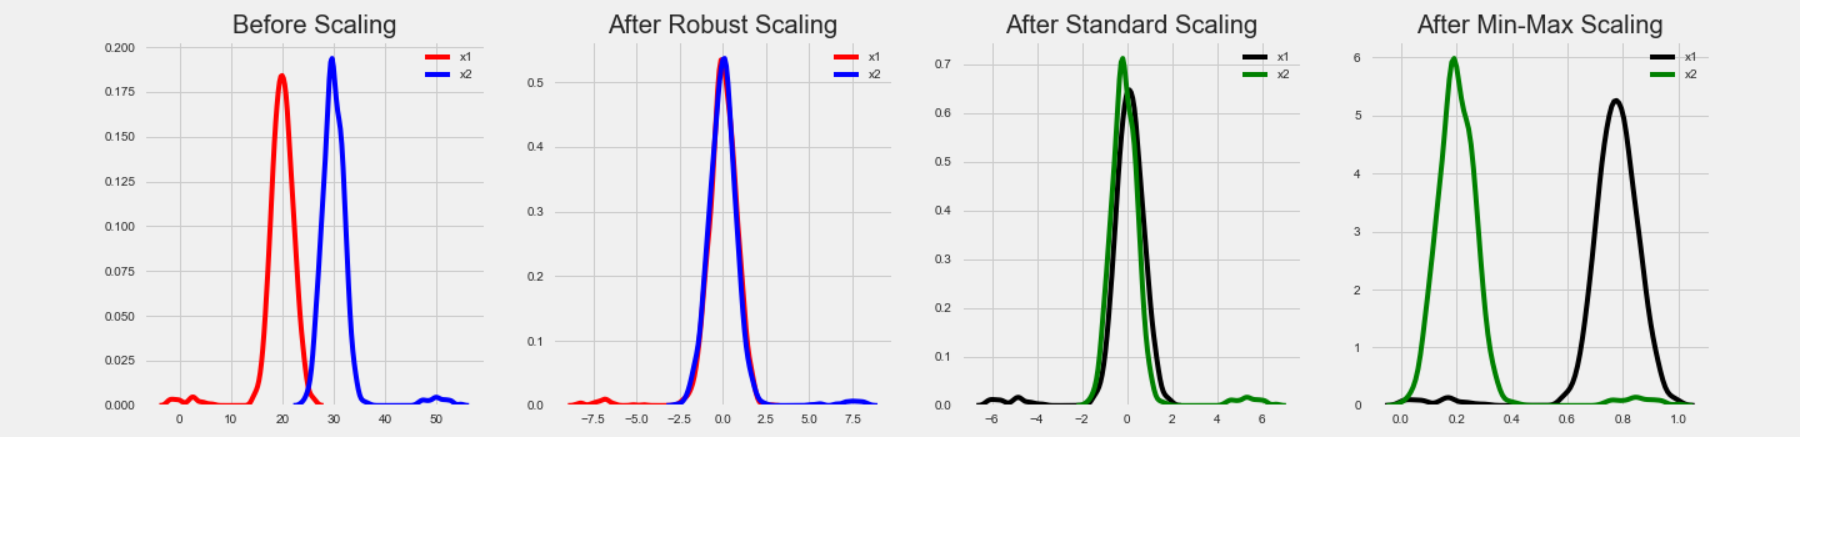
\includegraphics[scale=0.5]{scaler.png}
	\caption{from \href{https://www.geeksforgeeks.org/standardscaler-minmaxscaler-and-robustscaler-techniques-ml/}{Geeksfor geeks.}}
\end{figure}
\chapter{sklearn.pipeline}
The sklearn.pipeline module implements utilities to build a composite estimator, as a chain of transforms and estimators.

\chapter{sklearn.ensemble}
The sklearn.ensemble module includes ecnsemble-based methods for classification, regression and anomaly detection.
\section{sklearn.emsemble.RandomForestClassifier}


\chapter{sklearn.model\_selection}
See the Cross-validation: evaluating estimator performance, Tuning the hyper-parameters of an estimator and Learning curve sections for further details.
\begin{itemize}
	\item sklearn.model\_selection.train\_test\_split
\end{itemize}

\chapter{sklearn.metrics}
The sklearn.metrics module includes score functions, performance metrics and pairwise metrics and distance computations.

\begin{itemize}
	\item metrics.classification\_report
	\item metrics.confusion\_matrix
	\item metrics.roc\_curve
	\item metrics.roc\_auc\_score
\end{itemize}

\chapter{tf.keras.model}
Model groups layers into an object with training and inference features.
\chapter{ft.keras.layer}

\part{R.}
\chapter{ggplot}
\chapter{dplyr}
\chapter{tidyr} 

\part{SQL.}


\part{Julia.}

\part{C++.}

\nocite{*}
\bibliography{biblio.bib} 
\bibliographystyle{ieeetr}

\end{document}